% Book pp. 166-171 (PDF pp. 167-172)
\section{Deducing the Relation of Various Loci Under Given Condition}

\subsection{Locus}

A locus (plural $=$ loci) is a set of points which satisfies a given condition or
criterion. The result of a locus will either be a complete circle, a part of a circle
(arc), a line or a single point. Here, we will learn about some conditions or criteria
a set of points satisfies.

\textbf{Condition 1:}

The Locus of points are \textbf{equidistant} from one point.

The result of this locus is a circle which will be r units away from the given point.
The given point is the centre of the circle. The criterion or the condition is that:
``it is equidistant from the centre''

Figure 4.28 shows the locus of all points r units from point (h, k)
\begin{center}
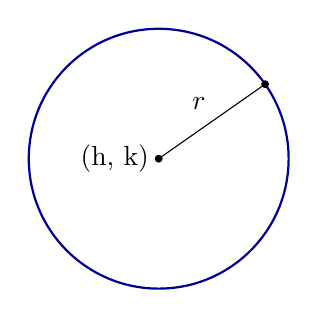
\begin{tikzpicture}[scale=1.1]
  \draw[blue!60!black, thick] (0,0) circle (1.5);
  \fill[black] (0,0) circle (1.3pt);
  \fill[black] (35:1.5) circle (1.3pt);
  \draw[black] (0,0) -- (35:1.5);
  \node[left] at (0,0) {(h, k)};
  \node[above left] at (35:0.8) {$r$};
\end{tikzpicture}
\end{center}
\figcaption{4.28}{Locus of all points r units from point (h, k)}

\begin{example}{Example 4.14}
Find the equation of all points 4 units away from $(-1, 2)$

\solution
This is the same as finding the equation of a circle with centre $(-1, 2)$ and radius
$= 4$.

Using the general equation of the circle, we have:
\booknote[S4-14]{it is the standard equation $(x - h)^2 + (y - k)^2 = r^2$ that is
used here, not the general equation.}
\begin{align*}
(x - (-1))^2 + (y - 2)^2 &= 4^2 \\
(x + 1)^2 + y^2 - 4y + 4 &= 16 \\
x^2 + 2x + 1 + y^2 - 4y + 4 &= 16 \\
x^2 + y^2 + 2x - 4y + 1 + 4 - 16 &= 0
\end{align*}
$\boldsymbol{x^2 + y^2 + 2x - 4y - 11 = 0}$ is the locus of all points 4 units away from the point
$(-1, 2)$
\end{example}

\textbf{Condition 2:}

The locus of points equidistant from two fixed points.

The result of this locus is a line which will perpendicularly bisect the line joining
the two points.

Figure 4.29 below shows the locus of points, L, equidistant from points P and Q.
Line L bisects PQ perpendicularly at m, the midpoint of line PQ.
\begin{center}
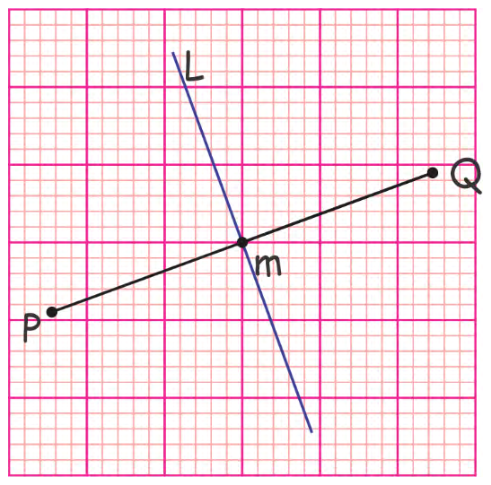
\includegraphics[width=0.4\linewidth]{figures/fig4-29.png}
\end{center}
\figcaption{4.29}{Locus of points, L, equidistant from points P and Q}

\begin{example}{Example 4.15}
Calculate the equation of all points equidistant from A(-5, 0) and B(3, -6)

\solution
\begin{align*}
\text{Midpoint of line AB} &= \left(\frac{-5 + 3}{2}, \frac{0 + -6}{2}\right) \\
&= \left(-\frac{2}{2}, -\frac{6}{2}\right) \\
&= (-1, -3)
\end{align*}
\begin{align*}
\text{Gradient of line AB} &= \frac{-6 - 0}{3 \text{ --- } 5} \\
&= -\frac{6}{8} \\
&= -\frac{3}{4}
\end{align*}
\begin{align*}
\text{Gradient of the locus} &= -1 \div \left(-\frac{3}{4}\right) \\
&= -1 \times -\frac{4}{3} \\
&= \frac{4}{3}
\end{align*}
Equation of the locos is:
\begin{align*}
y - -3 &= \frac{4}{3}(x - (-1)) \\
y + 3 &= \frac{4}{3}(x + 1)
\end{align*}
Multiply through by 3:
\begin{align*}
3 \times (y + 3) &= 3 \times \frac{3}{4}(x + 1) \\
3y + 9 &= 4(x + 1) \\
3y + 9 &= 4x + 4 \\
3y - 4x + 9 - 4 &= 0 \\
3y - 4x + 5 &= 0
\end{align*}
Therefore, $3\boldsymbol{y} - 4\boldsymbol{x} + 5 = 0$ is the locus of all points equidistant from (-5, 0) and
(3, -6)
\end{example}

\textbf{Condition 3:}

The locus of points equidistant from two intersecting lines.

The result of this locus is a pair of angle bisectors. For any point (x, y) on the
angle bisector, the perpendicular distance is equidistant from the two lines.

In Figure 4.30, l and m are the loci equidistant from line AB and line CD.

Line L bisects angle BOD and M bisects angle AOD.

Also, for any point P(x, y) on the locus, L, the perpendicular distance between
point P and line AB is equal to the perpendicular distance between point P and
line CD.
\begin{center}
\begin{tikzpicture}[scale=1.0, font=\scriptsize]
  \coordinate (O) at (0,0);
  % line AB: direction 165 deg (A upper left) to -15 deg (B lower right)
  \draw[black] (165:3.4) node[above left] {A} -- (-15:3.4) node[right] {B};
  % line CD: direction 215 deg (C lower left) to 35 deg (D upper right)
  \draw[black] (215:3.2) node[below left] {C} -- (35:3.2) node[above right] {D};
  % bisector L of angle BOD: direction 10 deg
  \draw[red] (190:3.6) -- (10:4.2) node[above] {L};
  % bisector m of angle AOD: direction 100 deg
  \draw[green!60!black] (280:1.6) -- (100:2.8) node[right] {m};
  \fill[black] (O) circle (1pt);
  \node[below right] at (O) {O};
  % P on m
  \coordinate (P1) at (100:2.1);
  \fill[blue!60!black] (P1) circle (1.2pt);
  \node[blue!60!black, right] at (P1) {P(x, y)};
  \draw[blue!60!black] (P1) -- ($(165:3.4)!(P1)!(-15:3.4)$);
  \draw[blue!60!black] (P1) -- ($(215:3.2)!(P1)!(35:3.2)$);
  % P on L
  \coordinate (P2) at (10:1.7);
  \fill[blue!60!black] (P2) circle (1.2pt);
  \node[blue!60!black, right] at (P2) {P(x, y)};
  \draw[cyan!70!black] (P2) -- ($(165:3.4)!(P2)!(-15:3.4)$);
  \draw[cyan!70!black] (P2) -- ($(215:3.2)!(P2)!(35:3.2)$);
\end{tikzpicture}
\end{center}
\figcaption{4.30}{Locus of points equidistant from two intersecting lines}

\begin{example}{Example 4.16}
Find the equation of the locus of points which moves so that its distance from the
lines

$y = 2x - 3$ and $x + 2y = 5$ is the same.

Let P(x, y) be any point on the loci. This means that the perpendicular distance
between P(x, y) and the line $y = 2x - 3$ is equal to the perpendicular distance
between point P(x,y) and the line $x + 2y = 5$

Recall that the perpendicular distance between a point (m,n) and a line $ax + by
+ c = 0$ is
\[ \left|\frac{a(m) + b(n) + c}{\sqrt{a^2 + b^2}}\right| \]
The equation of the loci is given by:
\begin{align*}
\left|\frac{y - 2x + 3}{\sqrt{1^2 + (-2)^2}}\right| &= \left|\frac{2y + x - 5}{\sqrt{2^2 + 1^2}}\right| \\
\left|\frac{y - 2x + 3}{\sqrt{5}}\right| &= \left|\frac{2y + x - 5}{\sqrt{5}}\right|
\end{align*}
multiply both sides by $\sqrt{5}$,which effectively removes the denominator:
\[ |y - 2x + 3| = |2y + x - 5| \]
Remove the absolute value sign by multiplying \textbf{any side} of the equation by $\pm$

In this example, we chose to remove the absolute value sign by multiplying the
RHS of the equation by $\pm$
\[ y - 2x + 3 = \pm(2y + x - 5) \]
So, either
\begin{center}
\begin{tabular}{@{}l@{\qquad}c@{\qquad}l@{}}
$y - 2x + 3 = 2y + x - 5$ & or & $y - 2x + 3 = -2y - x + 5$ \\
$0 = 2y - y + x + 2x - 5 - 3$ & & $y + 2y - 2x + x + 3 - 5 = 0$ \\
$y + 3x - 8 = 0$ & & $3y - x - 2 = 0$
\end{tabular}
\end{center}
Therefore, the equation of the locus is either $\boldsymbol{y} + 3\boldsymbol{x} - 8 = 0$ \textbf{or} $3\boldsymbol{y} - \boldsymbol{x} - 2 = 0$
\end{example}

\textbf{Condition 4:}

The locus equidistant from a line.

The result of this locus is a pair of lines equidistant from the given line.

For instance, the locus of points $\boldsymbol{d}$ units away from line AB is either line M or line
L as shown in Figure 4.31.
\begin{center}
\begin{tikzpicture}[scale=1.0, font=\small]
  \draw[black] (-2.2,-0.3) node[left] {A} -- (2.2,0.3) node[right] {B};
  \draw[red] (-2.0,0.45) -- (2.2,1.05) node[above] {L};
  \draw[blue!60!black] (-2.0,-1.05) -- (2.2,-0.45) node[right] {M};
  \draw[{Stealth}-{Stealth}] (-0.6,-0.083) -- (-0.7,0.62);
  \draw[{Stealth}-{Stealth}] (-0.1,-0.014) -- (-0.2,-0.79);
  \node[cyan!70!black, right] at (-0.6,0.3) {d};
  \node[cyan!70!black, right] at (-0.1,-0.4) {d};
\end{tikzpicture}
\end{center}
\figcaption{4.31}{Locus equidistant from a line}

So, if the equation of AB is $ax + by + c = 0$, then $d = \left|\dfrac{ax + by + c}{\sqrt{a^2 + b^2}}\right|$

\begin{example}{Example 4.17}
Find the locus of the point R(x, y) such that it is always 3 units from the line $y + 1 = 0$

\solution
\begin{align*}
3 &= \left|\frac{0x + y + 1}{\sqrt{0^2 + 1^2}}\right| \\
3 &= \left|\frac{y + 1}{\sqrt{1}}\right| \\
3 &= \pm|y + 1| \\
3 &= y + 1 \text{ or } 3 = -y - 1 \\
y - 2 &= 0 \text{ or } y + 4 = 0
\end{align*}
Therefore, the locus R($x$, $y$) of points which is 3 units away from $y + 1 = 0$ is
either $\boldsymbol{y} - 2 = 0$ \textbf{or} $\boldsymbol{y} + 4 = 0$
\end{example}

\begin{example}{Example 4.18}
If P(1, 4) and Q(5, -1) are two fixed points and A(x,y) moves such that $|$AP$|$:$|$AQ$|$
$= 1$:2. Find the equation of the locus.

\solution
From the condition given, $|$AP$|$:$|$AQ$| = 1 : 2$
\begin{align*}
\frac{|AP|}{|AQ|} &= \frac{1}{2} \\
2|AP| &= 1 \times |AQ| \\
2\sqrt{(y - 4)^2 + (x - 1)^2} &= \sqrt{(y - (-1))^2 + (x - 5)^2} \\
2\sqrt{(y - 4)^2 + (x - 1)^2} &= \sqrt{(y + 1)^2 + (x - 5)^2}
\end{align*}
Square both sides:
\begin{align*}
4\left[y^2 - 8y + 16 + x^2 - 2x + 1\right] &= y^2 + 2y + 1 + x^2 - 10x + 25 \\
4y^2 - 32y + 64 + 4x^2 - 8x + 4 &= y^2 + 2y + 1 + x^2 - 10x + 25 \\
4y^2 - y^2 - 32y - 2y + 4x^2 - x^2 - 8x + 10x + 68 - 26 &= 0
\end{align*}
$3\boldsymbol{x}^2 + 3\boldsymbol{y}^2 + 2\boldsymbol{x} - 34\boldsymbol{y} + 42 = 0$ is the equation of the locus.
\end{example}

\begin{example}{Example 4.19}
A point A(x, y) moves such that AC and AD are perpendicular.

If C(-3, 0) and D(3, 5), find the equation of the locus A.

\solution
Since AC and AD are perpendicular, (gradient of AC)$\times$ (gradient of AD)$= -1$
\begin{align*}
\left(\frac{y - 0}{x - (-3)}\right) \times \left(\frac{y - 5}{x - 3}\right) &= -1 \\
\left(\frac{y}{x + 3}\right) \times \left(\frac{y - 5}{x - 3}\right) &= -1 \\
\frac{y^2 - 5y}{x^2 - 9} &= -\frac{1}{1}
\end{align*}
Cross multiply:
\begin{align*}
y^2 - 5y &= -1(x^2 - 9) \\
y^2 - 5y &= -x^2 + 9
\end{align*}
$\boldsymbol{y^2 + x^2 - 5y - 9 = 0}$ is the locus A
\end{example}

\section{Extended Reading}
\begin{itemize}
  \item Mathematical Association of Ghana (2009). Effective Elective Mathematics:
  Seddco Publishing Limited. ISBN 978 9964 72 4740.
\end{itemize}
